\documentclass{standalone}

\usepackage{tikz}
\usetikzlibrary{backgrounds, positioning, shapes.symbols}
\usepackage{helvet}
\renewcommand*{\rmdefault}{\sfdefault}

\begin{document}
\begin{tikzpicture}
  [
    font=\footnotesize,
    faraday/.style={minimum size=3cm, draw, dashed},
    duplexer/.style={draw,fill=white},
  ]

  \node[label=above:avra] (avra)
    {
\includegraphics[width=1.2cm]{server}};
  \node[right=0.5cm of avra, label=above:AW2S] (aw2s)
    {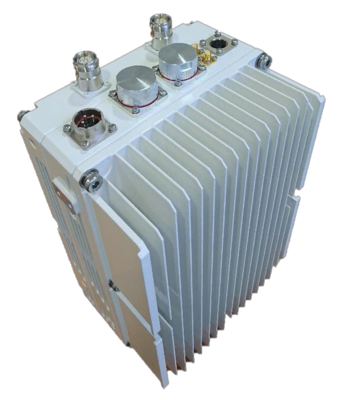
\includegraphics[width=1.2cm]{aw2s}} edge (avra);
  \node[right=.2cm of aw2s, duplexer] (b78o) {n78} edge (aw2s);
  \node[above right=-0.7cm and 0.35cm of b78o.east] (anto1)
    {
\includegraphics[width=0.3cm]{antenna}} edge (b78o);
  \node[below right=-0.7cm and 0.35cm of b78o.east] (anto2)
    {
\includegraphics[width=0.3cm]{antenna}} edge (b78o);

  \node[right=4cm of aw2s, label=above:Amarisoft UE] (amariue)
    {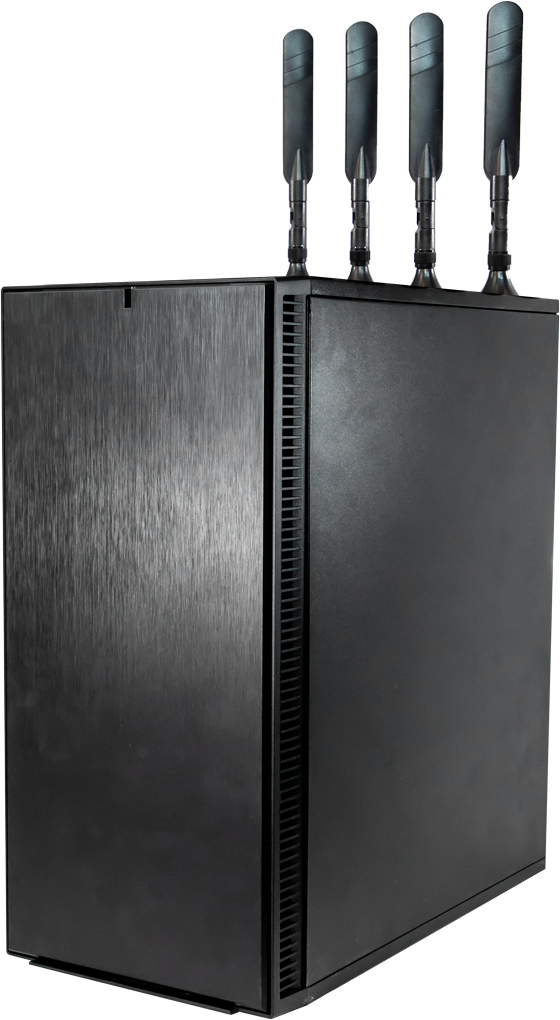
\includegraphics[width=0.7cm]{amariue}};
  \node[right=3cm of aw2s] (anto3)
    {
\includegraphics[width=0.3cm]{antenna}} edge (amariue);

\end{tikzpicture}
\end{document}
